\documentclass{oci}
\usepackage[utf8]{inputenc}
\usepackage{lipsum}

%\DeclareUnicodeCharacter{1F44D}{\thumbsup}
\newcommand{\thumbsup}{\raisebox{-0.1em}{
\includegraphics[scale=0.18]{thumbsup.png}}}
\newcommand{\onehundred}{\raisebox{-0.1em}{
\includegraphics[scale=0.18]{100.png}}}
\newcommand{\fire}{\raisebox{-0.1em}{
\includegraphics[scale=0.18]{fire.png}}}

\title{Reacciones}

\newcommand{\platform}{Ocimatic}
\newcommand{\hero}{Francisca}

\begin{document}
\begin{problemDescription}
\platform{} es una conocida plataforma de mensajería instantánea
por texto.
% en la que los usuarios pueden comunicarse entre pares o grupos.
%
Una sus funcionalidades más populares es la posibilidad de \emph{reaccionar}
con emojis a los mensajes de otros participantes.
%
Específicamente, un usuario puede reaccionar con uno o más emojis,
pero solo una vez con cada emoji.

Las reacciones se muestran en una lista horizontal
debajo de los mensajes.
%
Asociado a cada reacción hay un contador.
%
Si se reacciona con un emoji que ya había sido utilizado previamente,
su contador aumenta en uno.
%
En caso de reaccionar con un nuevo emoji, este se agrega al final de la lista con
un contador igual a 1.
%
Por ejemplo, en la imagen de la izquierda que se muestra
a continuación hay 5 reacciones con el emoji \thumbsup{} y 2 reacciones
con \onehundred{}.
%
Ya que el emoji \fire{} no ha sido utilizado aún, al reaccionar con este
se añade a la lista como se muestra en la imagen de la derecha.
\begin{center}
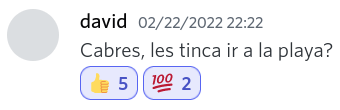
\includegraphics[scale=0.5]{reactions1.png}
\hspace{6em}
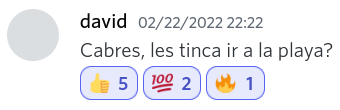
\includegraphics[scale=0.5]{reactions2.png}
\end{center}

\hero{} es una usuaria frecuente de \platform{}.
%
Una de sus costumbres es usar las reacciones para
escribir mensajes.
%
Esto es posible en algunos casos ya que \platform{}
tiene emojis por cada letra del abecedario en $k$ colores diferentes.
%
Si \hero{} reacciona con estos emojis en el orden adecuado
entonces puede escribir algunos mensajes.
%
La siguiente imagen muestra como \hero{} puede usar las reacciones para
escribir \texttt{excelente}.
%
Para esto, debe reaccionar con la letra \texttt{e} en cuatro colores distintos.
%
\begin{center}
  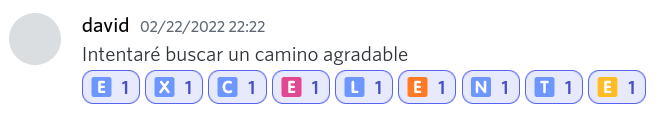
\includegraphics[scale=2.2]{reactions3.png}
\end{center}

A \hero{} le gustaría poder determinar si es posible o no formar un mensaje
usando las reacciones antes de intentar escribirlo, de lo contrario,
podría ocurrir que empiece a formar el mensaje y quede incompleto, afectando
así su reputación en \platform{}.
%
?`Podrías ayudarla?

\end{problemDescription}

\begin{inputDescription}
La primera línea de la entrada contiene dos enteros $n$ y $k$ ($1 \le k \le n \le 1\,000\,000$)
que corresponden respectivamente al largo del mensaje que \hero{} quiere escribir
con emojis y al número de colores que \platform{} tiene por cada letra del abecedario.
%
Representaremos cada color con un entero entre 1 y $k$.

La segunda línea contiene un mensaje de largo $n$ formado por letras del abecedario
inglés (es decir, sin la \textbf{ñ}), en minúsculas y sin espacios.
\end{inputDescription}

\begin{outputDescription}
La salida consiste en una sola línea.

Si existe una manera de formar el mensaje, la línea debe contener $n$
enteros $c_i$ ($1 \le c_i \le k$) separados por espacios,
donde el $i$-ésimo entero indica el color del que debe ser pintada la $i$-ésima
letra del mensaje.
%
Puedes imprimir cualquier secuencia de colores válida.
%
Una secuencia es válida si ninguna letra aparece dos veces con el
mismo color y cada color es un número válido entre 1 y $k$.

Si no es posible escribir el mensaje, la línea debe contener la palabra \texttt{imposible}.
\end{outputDescription}

\begin{scoreDescription}
  \subtask{20}
  Se probarán varios casos en que $k = 1$.
  \subtask{30}
  Se probarán varios casos en que $k = 2$.
  \subtask{50}
  Se probarán varios casos sin restricciones adicionales.
\end{scoreDescription}

\begin{sampleDescription}
\sampleIO{sample-1}
\sampleIO{sample-2}
\end{sampleDescription}

\end{document}
